\newpage{}

\section{Trigonometrie}
\subsection{Gradmass, Bogenmass}
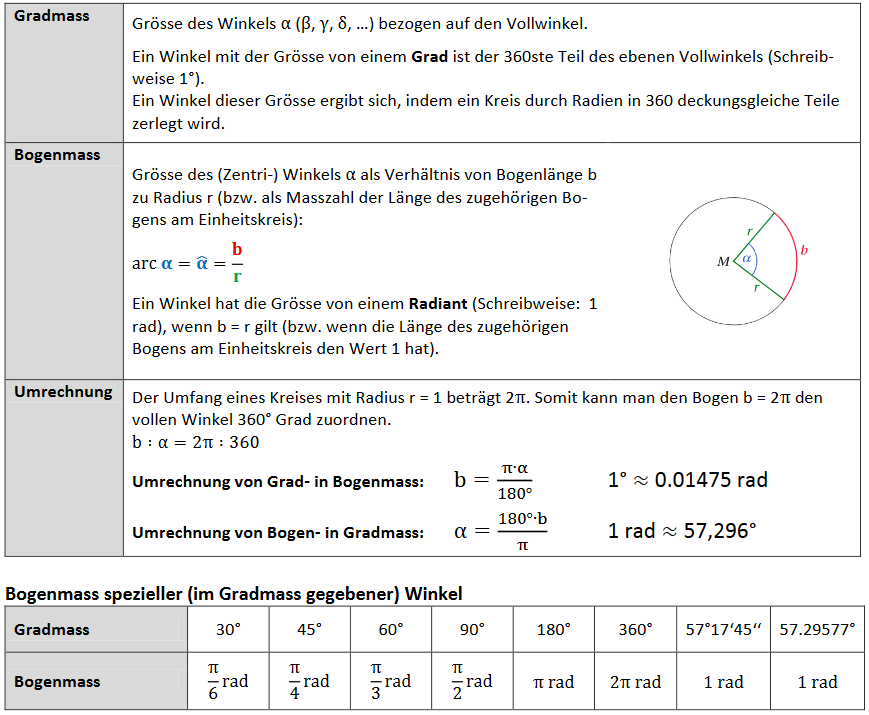
\includegraphics[scale=0.7]{gradmass.PNG}
\subsection{Trigonometrische Funktionen am rechtwinkligen Dreieck}
\subsubsection{Sinus, Kosekans}
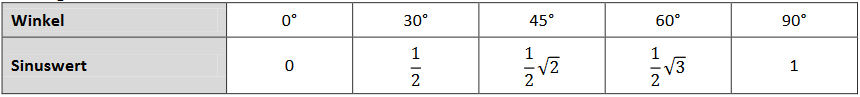
\includegraphics[scale=0.7]{sinkan1.PNG}

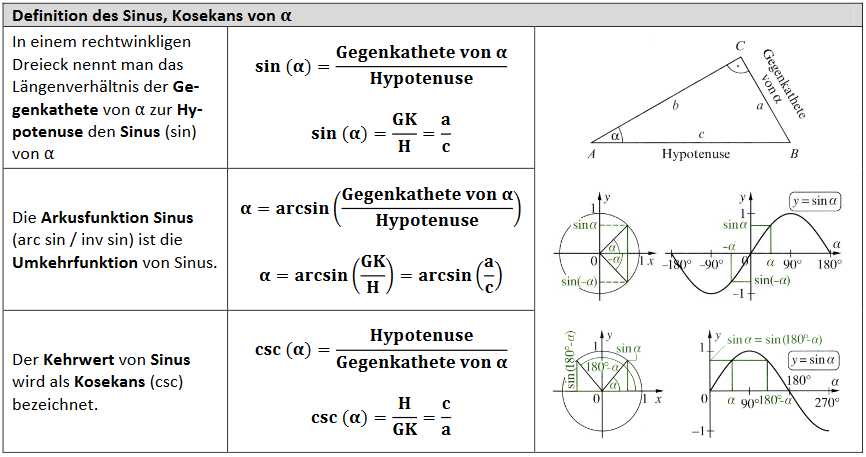
\includegraphics[scale=0.7]{sinkan2.PNG}
\subsubsection{Kosinus, Sekans}
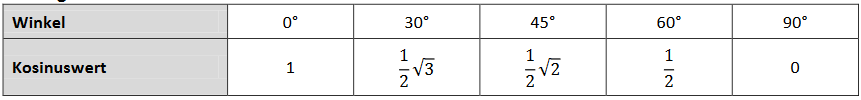
\includegraphics[scale=0.7]{kossek1.PNG}

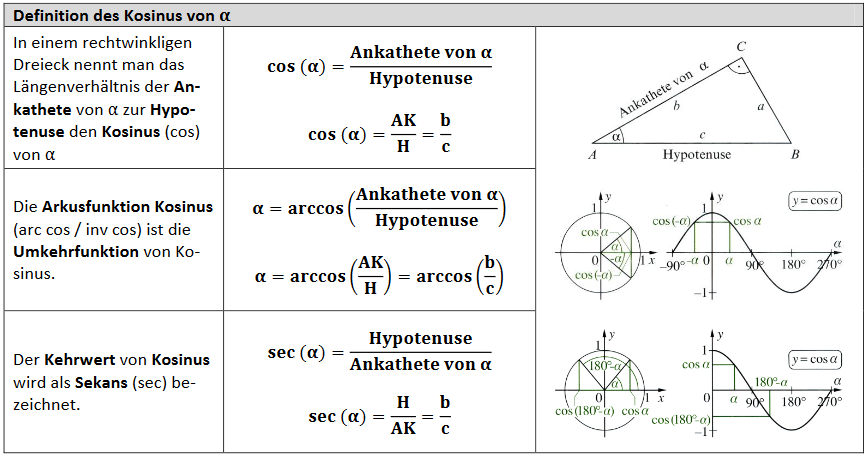
\includegraphics[scale=0.7]{kossek2.PNG}
\subsubsection{Tangens, Kotangens}
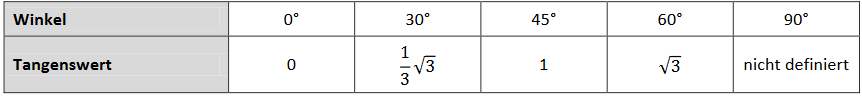
\includegraphics[scale=0.7]{tanko1.PNG}

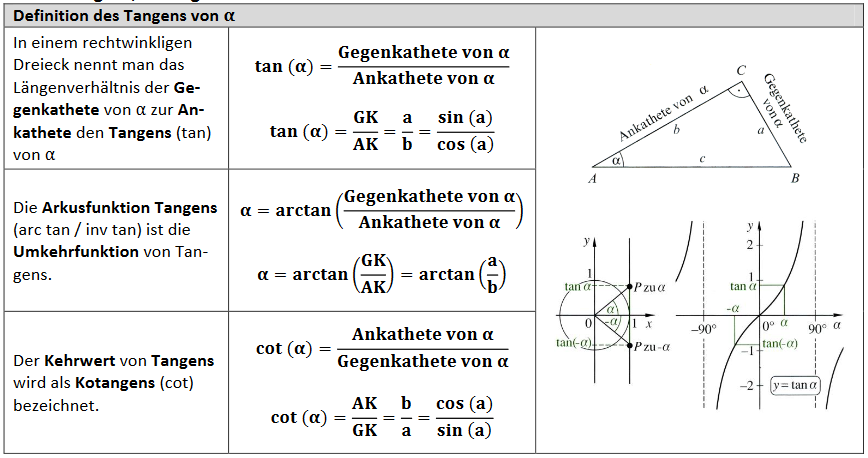
\includegraphics[scale=0.7]{tanko2.PNG}

\subsubsection{Sinus- Kosinus- und Tangensfunktion am rechtwinkligen Dreieck}
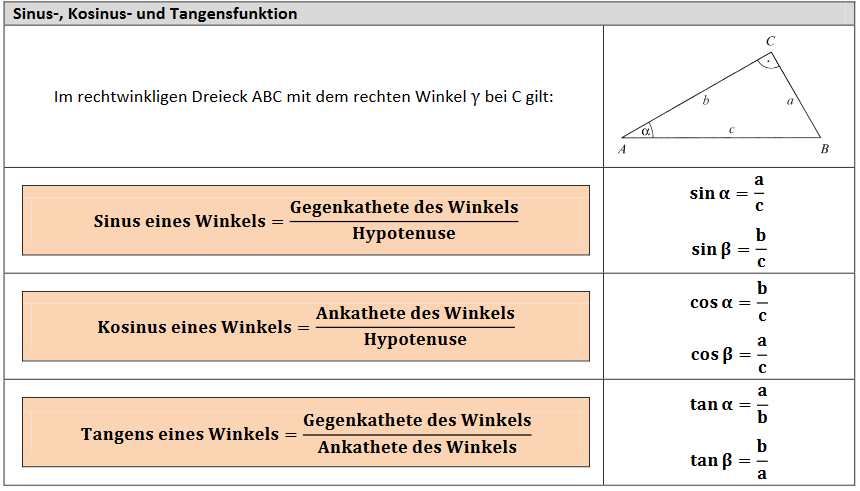
\includegraphics[scale=0.7]{sinkota.PNG}

\newpage{}


\subsection{Trigonometrische Funktionen am schiefwinkligen Dreieck}
\subsubsection{Kosinussatz}
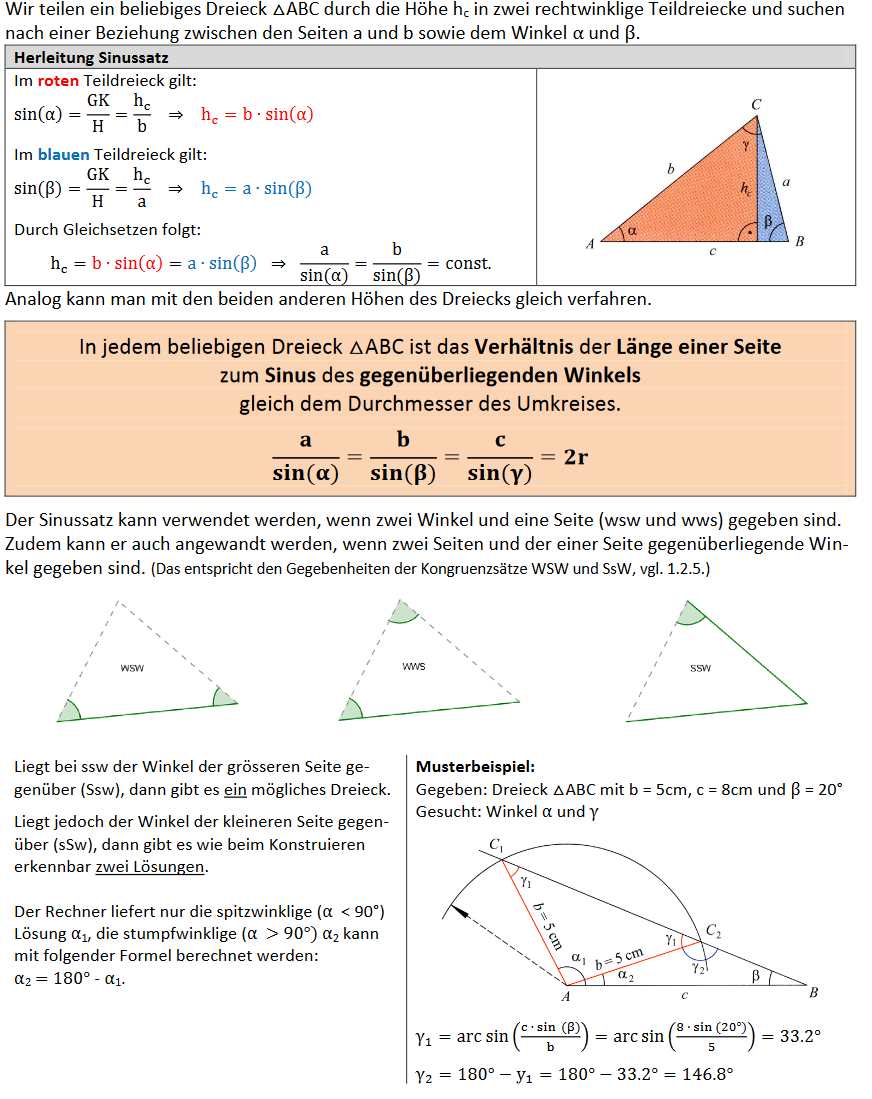
\includegraphics[scale=0.7]{sinussatz.PNG}
\subsubsection{Sinussatz}
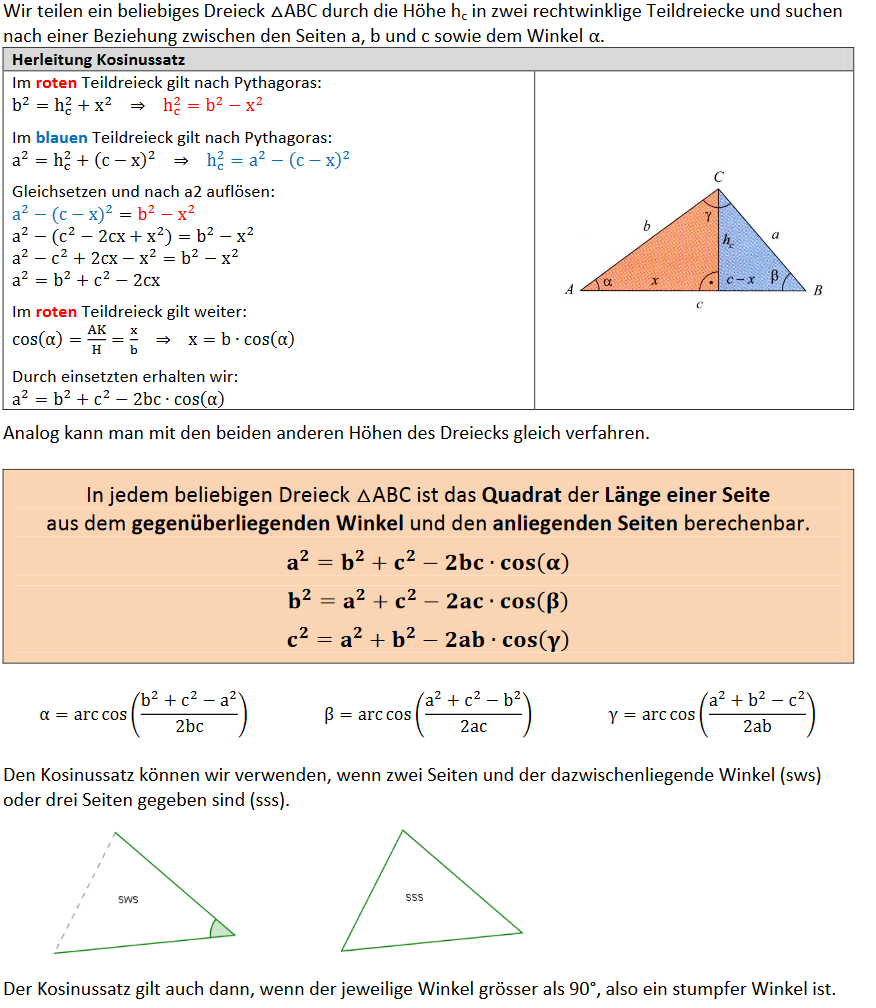
\includegraphics[scale=0.7]{kosinussatz.PNG}

\subsubsection{Flaechensatz}
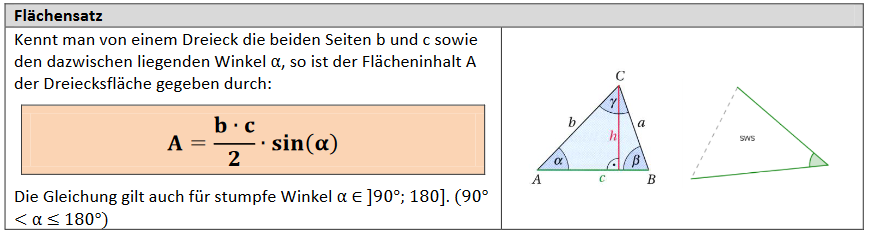
\includegraphics[scale=0.7]{flaechensatz.PNG}
\subsubsection{Berechnung am Kreissektor (auch Kreisausschnitt)}
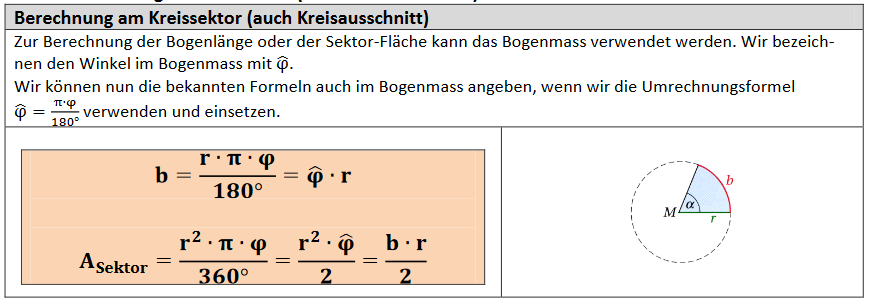
\includegraphics[scale=0.7]{kreissektor.PNG}
\subsubsection{Kreissegment (auch Kreisabschnitt)}
\includegraphics[scale=0.7]{kreissegment.PNG}



\subsection{Einheitskreis}
\subsubsection{Definition}
Der Einheitskreis ist ein Kreis um den Koordinatenursprung mit dem Radius r = 1 Längeneinheit.
\subsubsection{Beziehungen zwischen den Winkelfunktionen (Phytagoras am Einheitskreis)}
\begin{multicols}{2}
    Pythagoras am Einheitskreis:
    \[\sin^2(a)+\cos^2(a)=1\]
    Ähnlichkeiten am Einheitskreis:
    \[\tan(a)=\frac{\sin(a)}{\cos(a)}\]
    \[\cot(a)=\frac{\cos(a)}{\sin(a)}\]
    \[\tan(a)+\cot(a)=1\]


    \begin{tikzpicture}[scale=1.9]
        \draw[step=.5cm,gray,very thin] (-1.4,-1.4) grid (1.4,1.4);
        \filldraw[fill=blue!20,draw=red] (0,0) -- (3mm,0mm)
        arc [start angle=0, end angle=30, radius=3mm] -- cycle;
        \node[red] at (15:2mm) {$\alpha$};
        \draw[->] (-1.5,0) -- (1.5,0) coordinate (x axis)node[right]{$0^\circ $};
        \draw[->] (0,-1.5) -- (0,1.5) coordinate (y axis)node[above]{$90^\circ$};
        \draw[->] (1.5,0) -- (-1.5,0) coordinate (x axis)node[left]{$180^\circ$};
        \draw[->] (0,1.5) -- (0,-1.5) coordinate (y axis)node[below]{$270^\circ$};
        \draw (0,0) circle [radius=1cm];
        \draw[very thick,orange]
        (30:1cm) -- node[left=1pt,fill=white] {$\sin \alpha$} (30:1cm |- x axis);
        \draw[very thick,blue]
        (30:1cm |- x axis) -- node[below=2pt,fill=white] {$\cos \alpha$} (0,0);
        \path [name path=upward line] (1,0) -- (1,1);
        \path [name path=sloped line] (0,0) -- (30:1.5cm);
        \draw [name intersections={of=upward line and sloped line, by=t}]
        [very thick,red] (1,0) -- node [right=1pt,fill=white]
        {$\displaystyle \tan \alpha$} (t);
        \draw (0,0) -- (t);

    \end{tikzpicture}
\end{multicols}
\begin{tabularx}{1\textwidth} {
        | >{\raggedright\arraybackslash}c
        | >{\raggedright\arraybackslash}X
        | >{\raggedright\arraybackslash}X
        | >{\raggedright\arraybackslash}X
        | >{\raggedright\arraybackslash}X |}
    \hline
                        & \boldmath $\sin(a)$                    & \boldmath $\cos(a)$                    & \boldmath $\tan(a)$                    & \boldmath $\cot(a)$                    \\\hline
    \boldmath $\sin(a)$ &                                        & $\sqrt[]{1-\cos^2(a)}$                 & $\frac{\tan(a)}{\sqrt[]{1+\tan^2(a)}}$ & $\frac{1}{\sqrt[]{1+\cot^2(a)}}$       \\ \hline
    \boldmath $\cos(a)$ & $\sqrt[]{1-\sin^2(a)}$                 &                                        & $\frac{1}{\sqrt[]{1+\tan^2(a)}}$       & $\frac{\cot(a)}{\sqrt[]{1+\cot^2(a)}}$ \\ \hline
    \boldmath $\tan(a)$ & $\frac{\sin(a)}{\sqrt[]{1-\sin^2(a)}}$ & $\frac{\sqrt[]{1-\cos^2(a)}}{\cos(a)}$ &                                        & $\frac{1}{\cot(a)}$                    \\ \hline
    \boldmath $\cot(a)$ & $\frac{\sqrt[]{1-\sin^2(a)}}{\sin(a)}$ & $\frac{\cos(a)}{\sqrt[]{1-\cos^2(a)}}$ & $\frac{1}{\tan(a)}$                    &                                        \\ \hline
\end{tabularx}
\subsubsection{Vorzeichen der Trigonometrischen Funktionen}
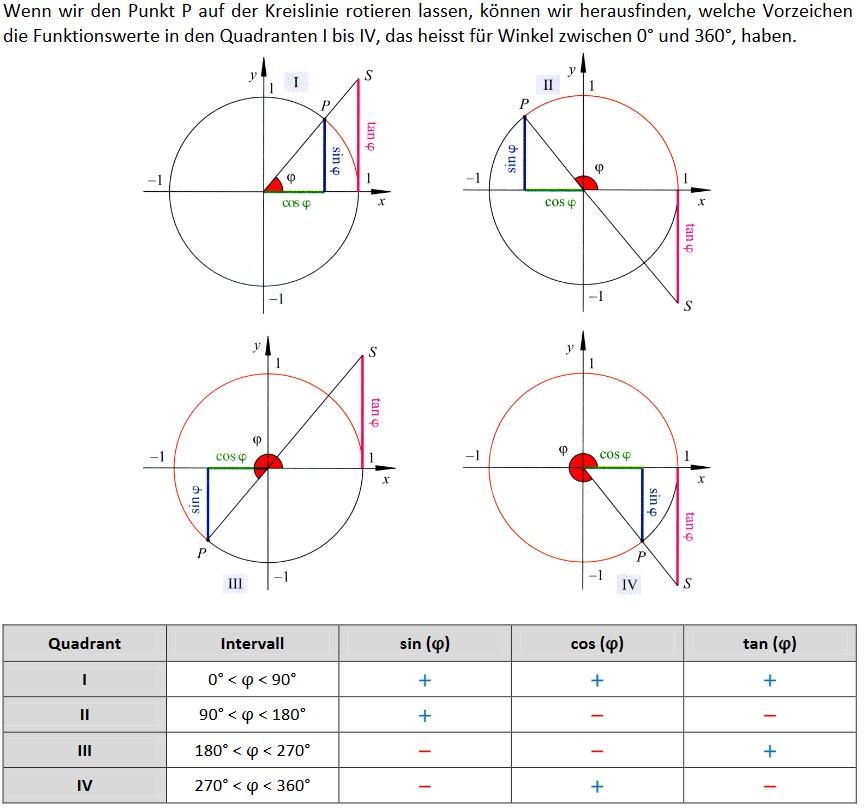
\includegraphics[scale=0.7]{einheitskreis4.PNG}

\subsection{Eigenschaften der Funktionen}
\begin{tabularx}{1\textwidth} {
        | >{\raggedright\arraybackslash}c
        | >{\raggedright\arraybackslash}X
        | >{\raggedright\arraybackslash}X
        | >{\raggedright\arraybackslash}X |}
    \hline
                                & \textbf{Sinus}                                                       & \textbf{Kosinus}                                                             & \textbf{Tangens}                                                                       \\\hline
    \textbf{Definitionsbereich} & $\left\{ x|x\in\mathbb{R}\right\}$ or $\left(-\infty,+\infty\right)$ & $\left\{ x|x\in\mathbb{R}\right\}$ or $\left(-\infty,+\infty\right)$         & $\mathbb{D}_f = \mathbb{R}\setminus\{\tfrac{\pi}{2} + k \cdot \pi, k \in \mathbb{Z}\}$ \\ \hline
    \textbf{Wertebereich}       & $\left[-1,1\right]$                                                  & $\left[-1,1\right]$                                                          & $\mathbb{W}_f = \mathbb{R}$                                                            \\ \hline
    \textbf{Periodizität}       & $2\pi$                                                               & $2\pi$                                                                       & $\pi$                                                                                  \\ \hline
    \textbf{Symmetrie}          & Punktsymetrisch zum Ursprung: Ungerade Funktion $\sin(-x)=-\sin(x)$  & Symetrisch zur y-Achse: gerade Funktion $\cos(x) = \cos(-x)$                 & Punktsymetrisch zum Ursprung: Ungerade Funktion $\tan(-x)=-\tan(x)$                    \\ \hline
    \textbf{Symmetrieachsen}    & $x=\frac{\pi}{2}+k\cdot \pi$ $k \in Z$                               & $x=k\cdot \pi$ $k \in Z$                                                     & $k \cdot \pi$                                                                          \\ \hline
    \textbf{Nullstellen}        & $x_k = k \cdot \pi$ $k \in \mathbb{Z}$                               & $x_k = \frac{\pi}{2} + k \cdot \pi$ $k \in \mathbb{Z}$    $k \in \mathbb{Z}$ & $x_k = k \cdot \pi$   $k \in \mathbb{Z}$                                               \\ \hline
    \textbf{Maxima}             & $x_k = \frac{\pi}{2} + k \cdot 2\pi$                                 & $x_k = k \cdot 2\pi$                                                         &                                                                                        \\ \hline
    \textbf{Minima}             & $x_k = \frac{3\pi}{2} + k \cdot 2\pi$                                & $x_k = \pi + k \cdot 2\pi$                                                   &                                                                                        \\ \hline
    \textbf{Es gilt}            & $\sin(x)=(\cos(x-\frac{\pi}{2})$)                                    & $\cos(x)=(\sin(x+\frac{\pi}{2})$)                                            & $\tan(x)=\frac{\sin(x)}{\cos(x)}$                                                      \\ \hline
\end{tabularx}

\newpage
\subsubsection{Identitäten}
\begin{multicols}{2}

    \textbf{Kofunktionen}
    \begin{align*}
         & \sin(\frac{\pi}{2} - x) & = \cos x \\
         & \cos(\frac{\pi}{2} - x) & = \sin x \\
         & \tan(\frac{\pi}{2} - x) & = \cot x \\
         & \cot(\frac{\pi}{2} - x) & = \tan x \\
         & \sec(\frac{\pi}{2} - x) & = \csc x \\
         & \csc(\frac{\pi}{2} - x) & = \sec x
    \end{align*}

    \textbf{Symmetrie}
    \begin{align*}
        \sin(-x) & = - \sin x \\
        \cos(-x) & = \cos x   \\
        \tan(-x) & = -\tan x
    \end{align*}

    \textbf{Doppelter Winkel}
    \begin{align*}
        \sin(2x) & = 2 \sin x \cos x               \\
        \cos(2x) & = \cos^2 x - \sin^2 x           \\
                 & = 2 \cos^2 x - 1                \\
                 & = 1 - 2 \sin^2 x                \\
        \tan(2x) & = \frac{2 \tan x}{1 - \tan^2 x}
    \end{align*}

    \textbf{Halber Winkel}
    \begin{align*}
        \sin \frac{x}{2} & = \pm \sqrt{ \frac{1 - \cos x }{2} } \\
        \cos \frac{x}{2} & = \pm \sqrt{ \frac{1 + \cos x }{2} } \\
        \tan \frac{x}{2} & = \frac{1 - \cos x }{\sin x}         \\
                         & = \frac{ \sin x }{ 1 + \cos x }
    \end{align*}

    \textbf{Exponent Reduktion}
    \begin{align*}
        \sin^2 x & = \frac{1 - \cos 2x}{2}               \\
        \sin^4x  & = (\frac{1 - \cos 2x}{2})^2           \\
        \cos^2 x & = \frac{1 + \cos 2x}{2}               \\
        \cos^4x  & = (\frac{1 + \cos 2x}{2})^2           \\
        \tan^2 x & = \frac{1 - \cos 2x}{1 + \cos 2x}     \\
        \tan^4 x & =( \frac{1 - \cos 2x}{1 + \cos 2x})^2
    \end{align*}

    \textbf{Pythagoras}
    \begin{align*}
        \sin^2 x + \cos^2 x & = 1        \\
        1 + \tan^2 x        & = \sec^2 x \\
        1 + \cot^2 x        & = \csc^2 x
    \end{align*}

    \textbf{Umkehrwert}
    \begin{align*}
        \cot x & = \frac{1}{\tan x} \\
        \csc x & = \frac{1}{\sin x} \\
        \sec x & = \frac{1}{\cos x}
    \end{align*}

    \textbf{Summe und Differenz von Winkel}
    \begin{align*}
        \sin(x + y) & = \sin x \cos y + \cos x \sin y             \\
        \sin(x - y) & = \sin x \cos y - \cos x \sin y             \\
        \cos(x + y) & = \cos x \cos y - \sin x \sin y             \\
        \cos(x - y) & = \cos x \cos y + \sin x \sin y             \\
        \tan(x + y) & = \frac{\tan x + \tan y}{1 - \tan x \tan y} \\
        \tan(x - y) & = \frac{\tan x - \tan y}{1 + \tan x \tan y}
    \end{align*}

    \textbf{Produkt zu Summe}
    \begin{align*}
        \sin x \sin y & = \frac{1}{2}\big[\cos(x - y) - \cos(x + y)\big] \\
        \cos x \cos y & = \frac{1}{2}\big[\cos(x - y) + \cos(x + y)\big] \\
        \sin x \cos y & = \frac{1}{2}\big[\sin(x + y) + \sin(x - y)\big] \\
        \tan x \tan y & = \frac{ \tan x + \tan y }{ \cot x + \cot y }    \\
        \tan x \cot y & = \frac{ \tan x + \cot y }{ \cot x + \tan y }
    \end{align*}

    \textbf{Summe Zu Produkt}
    \begin{align*}
        \sin x + \sin y & = 2 \sin \Big( \frac{x + y}{2} \Big) \cos \Big( \frac{x - y}{2} \Big)  \\
        \sin x - \sin y & = 2 \cos \Big( \frac{x + y}{2} \Big) \sin \Big( \frac{x - y}{2} \Big)  \\
        \cos x + \cos y & = 2 \cos \Big( \frac{x + y}{2} \Big) \cos \Big( \frac{x - y}{2} \Big)  \\
        \cos x - \cos y & = -2 \sin \Big( \frac{x + y}{2} \Big) \sin \Big( \frac{x - y}{2} \Big) \\
        \tan x + \tan y & = \frac{ \sin(x + y) }{ \cos x \cos y}                                 \\
        \tan x - \tan y & = \frac{ \sin(x - y) }{ \cos x \cos y}                                 \\
    \end{align*}

\end{multicols}
\newpage
\begin{multicols}{2}
    \subsection{Transformation der Sinusfunktion}
    \subsubsection{Allgemeine Sinusfunktion}
    Die allgemeine Sinusfunktion ist folgendermassen definiert:
    \[y=a\cdot\sin(b\cdot(x+u))+v\]
    \subsubsection{Strecken und Stauchen auf y-Achse}
    Parameter a: Strecken / Stauchen auf y-Achse (Amplitude): $y=a\cdot\sin(x)$ $a\in\mathbb{R}_{0}$

    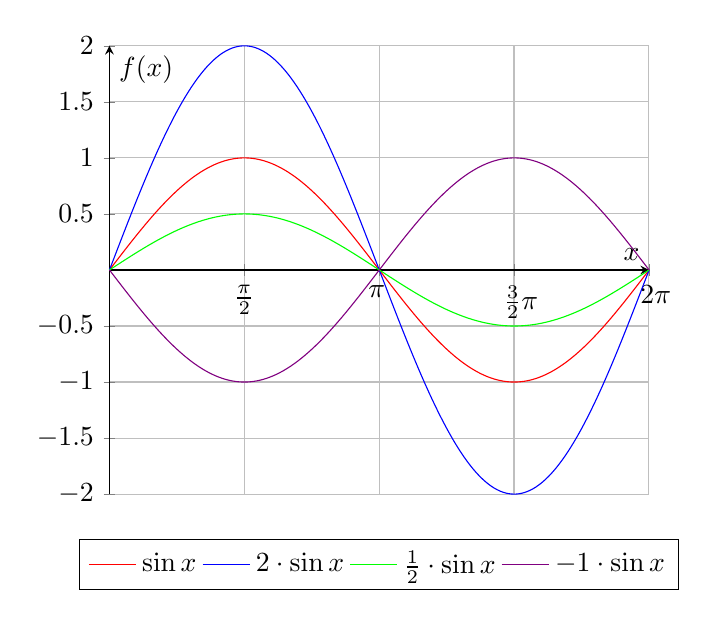
\begin{tikzpicture}
        \begin{axis}[
                clip=false,
                xmin=0,xmax=2*pi,
                xlabel= $x$,
                ylabel=$f(x)$,
                ymin=-2,ymax=2,
                ytick={-2,-1.5,-1,-0.5,0,0.5,1,1.5,2},
                axis lines=middle,
                grid,
                legend style={at={(0.5,-0.1)},
                        anchor=north,legend columns=-1},
                %axis x line=middle,
                %axis y line=left,
                %     axis x line=middle,
                xtick={0,1.57,3.14,4.71,6.28},
                xticklabels={$0$, $\frac{\pi}{2}$,$\pi\,$,$\,\,\,\frac{3}{2}\pi$,$\,\,\,2\pi$},
                %xticklabel style={anchor=north west}
            ]
            \addplot[domain=0:2*pi,samples=200,red]{sin(deg(x))};
            \addlegendentry {$\sin x$};
            \addplot[domain=0:2*pi,samples=200,blue]{2*(sin(deg(x)))};
            \addlegendentry {$2\cdot \sin x$};
            \addplot[domain=0:2*pi,samples=200,green]{0.5*(sin(deg(x)))};
            \addlegendentry {$\frac{1}{2}\cdot \sin x$};
            \addplot[domain=0:2*pi,samples=200,violet]{-1*(sin(deg(x)))};
            \addlegendentry {$-1\cdot \sin x$};
        \end{axis}
    \end{tikzpicture}

    \begin{tabularx}{0.5\textwidth} {
            >{\centering\arraybackslash}c
            >{\centering\arraybackslash}c
            >{\centering\arraybackslash}c}
        \boldmath $|a|>1$ & \boldmath$0<|a|<1$ & \boldmath$|a|<0$      \\
        Streckung         & Stauchung          & Spiegelung an x-Achse \\
    \end{tabularx}

    \subsubsection{Strecken und Stauchen auf x-Achse}
    Parameter b: Strecken / Stauchen auf x-Achse: $y=sin(b\cdot x)$ $b\in\mathbb{R}^{+}$

    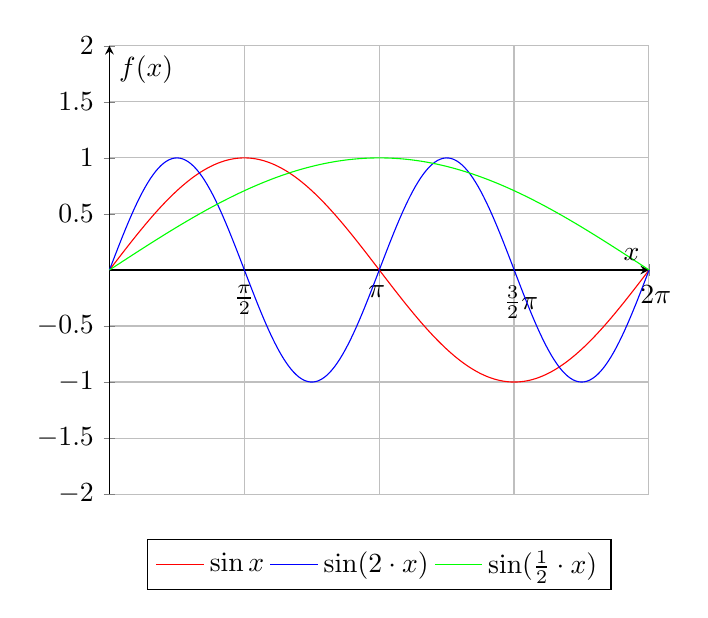
\begin{tikzpicture}
        \begin{axis}[
                clip=false,
                xmin=0,xmax=2*pi,
                xlabel= $x$,
                ylabel=$f(x)$,
                ymin=-2,ymax=2,
                ytick={-2,-1.5,-1,-0.5,0,0.5,1,1.5,2},
                axis lines=middle,
                grid,
                legend style={at={(0.5,-0.1)},
                        anchor=north,legend columns=-1},
                %axis x line=middle,
                %axis y line=left,
                %     axis x line=middle,
                xtick={0,1.57,3.14,4.71,6.28},
                xticklabels={$0$, $\frac{\pi}{2}$,$\pi\,$,$\,\,\,\frac{3}{2}\pi$,$\,\,\,2\pi$},
                %xticklabel style={anchor=north west}
            ]
            \addplot[domain=0:2*pi,samples=200,red]{sin(deg(x))};
            \addlegendentry {$\sin x$};
            \addplot[domain=0:2*pi,samples=200,blue]{sin(deg(2*x))};
            \addlegendentry {$\sin(2\cdot x)$};
            \addplot[domain=0:2*pi,samples=200,green]{sin(deg(0.5*x))};
            \addlegendentry {$\sin(\frac{1}{2}\cdot x)$};


        \end{axis}
    \end{tikzpicture}

    \begin{tabularx}{0.5\textwidth} {
            >{\centering\arraybackslash}X
            >{\centering\arraybackslash}X}
        \boldmath $b>1$                     & \boldmath$0< b <1$                                                                        \\
        Stauchung in x-Richtung um den Faktor b.
        (kleinere Periode, höhere Frequenz) & Streckung in x-Richtung um den Faktor $\frac{1}{b}$.(grössere Periode, kleinere Frequenz) \\
    \end{tabularx}



    \subsubsection{Schieben in x-Richtung}
    Parameter u: Schieben in x-Richtung: $y=\sin(x+u)$ $u\in\mathbb{R}$

    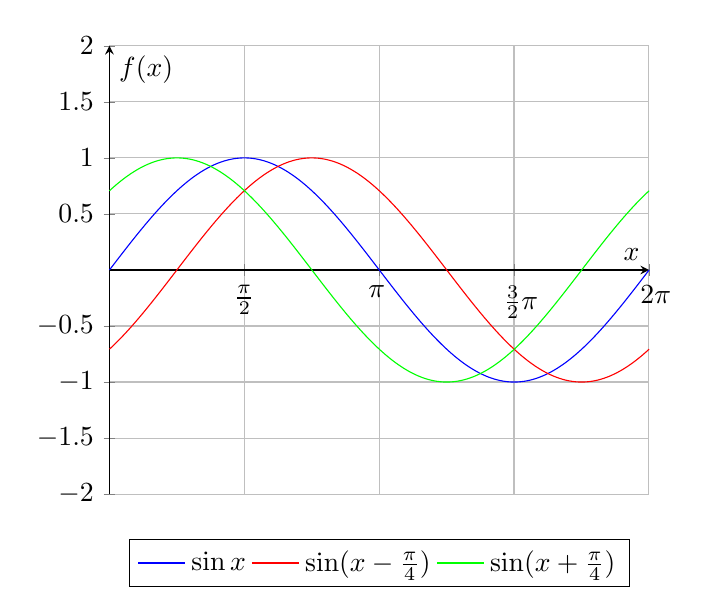
\begin{tikzpicture}
        \begin{axis}[
                clip=false,
                xmin=0,xmax=2*pi,
                xlabel= $x$,
                ylabel=$f(x)$,
                ymin=-2,ymax=2,
                ytick={-2,-1.5,-1,-0.5,0,0.5,1,1.5,2},
                axis lines=middle,
                grid,
                legend style={at={(0.5,-0.1)},
                        anchor=north,legend columns=-1},
                %axis x line=middle,
                %axis y line=left,
                %     axis x line=middle,
                xtick={0,1.57,3.14,4.71,6.28},
                xticklabels={$0$, $\frac{\pi}{2}$,$\pi\,$,$\,\,\,\frac{3}{2}\pi$,$\,\,\,2\pi$},
                %xticklabel style={anchor=north west}
            ]
            \addplot[domain=0:2*pi,samples=200,blue]{sin(deg(x))};
            \addlegendentry {$\sin x$};
            \addplot[domain=0:2*pi,samples=200,red]{(sin(deg(x-0.785)))};
            \addlegendentry {$\sin (x-\frac{\pi}{4})$};
            \addplot[domain=0:2*pi,samples=200,green]{(sin(deg(x+0.785)))};
            \addlegendentry {$\sin (x+\frac{\pi}{4})$};

        \end{axis}
    \end{tikzpicture}

    \begin{tabularx}{0.5\textwidth} {
            >{\centering\arraybackslash}X
            >{\centering\arraybackslash}X}
        \boldmath $u>1$          & \boldmath$u < 0$          \\
        Verschiebung nach links. & Verschiebung nach rechts. \\
    \end{tabularx}



    \subsubsection{Schieben in y-Richtung}
    Parameter v: Schieben in y-Richtung:  $y=a\cdot\sin(x)+v$ $v\in\mathbb{R}$

    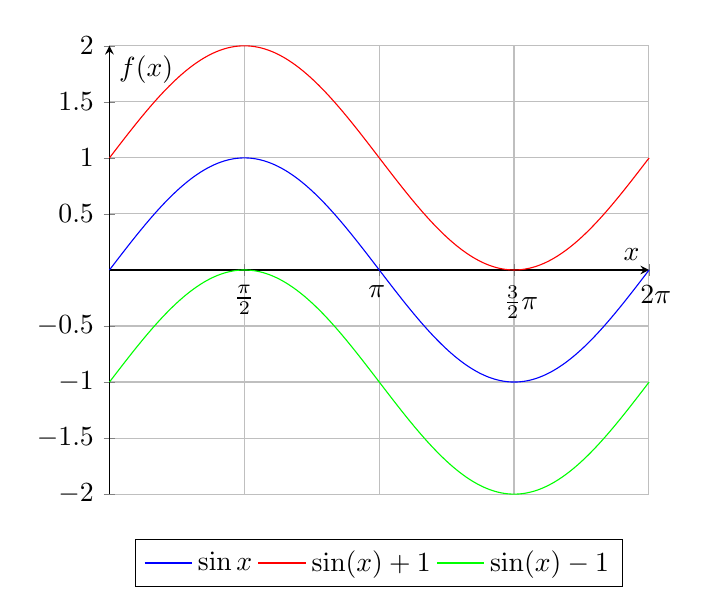
\begin{tikzpicture}
        \begin{axis}[
                clip=false,
                xmin=0,xmax=2*pi,
                xlabel= $x$,
                ylabel=$f(x)$,
                ymin=-2,ymax=2,
                ytick={-2,-1.5,-1,-0.5,0,0.5,1,1.5,2},
                axis lines=middle,
                grid,
                legend style={at={(0.5,-0.1)},
                        anchor=north,legend columns=-1},
                %axis x line=middle,
                %axis y line=left,
                %     axis x line=middle,
                xtick={0,1.57,3.14,4.71,6.28},
                xticklabels={$0$, $\frac{\pi}{2}$,$\pi\,$,$\,\,\,\frac{3}{2}\pi$,$\,\,\,2\pi$},
                %xticklabel style={anchor=north west}
            ]
            \addplot[domain=0:2*pi,samples=200,blue]{sin(deg(x))};
            \addlegendentry {$\sin x$};
            \addplot[domain=0:2*pi,samples=200,red]{(sin(deg(x))+1)};
            \addlegendentry {$\sin (x)+1$};
            \addplot[domain=0:2*pi,samples=200,green]{(sin(deg(x))-1)};
            \addlegendentry {$\sin (x)-1$};

        \end{axis}
    \end{tikzpicture}

    \begin{tabularx}{0.5\textwidth} {
            >{\centering\arraybackslash}X
            >{\centering\arraybackslash}X}
        \boldmath $v >1$        & \boldmath$v < 0$         \\
        Verschiebung nach oben. & Verschiebung nach unten. \\
    \end{tabularx}

\end{multicols}
\newpage{}





\newpage{}
\section{Goniometrie}
\subsection{Grundlagen}
\subsubsection{Beziehungen}
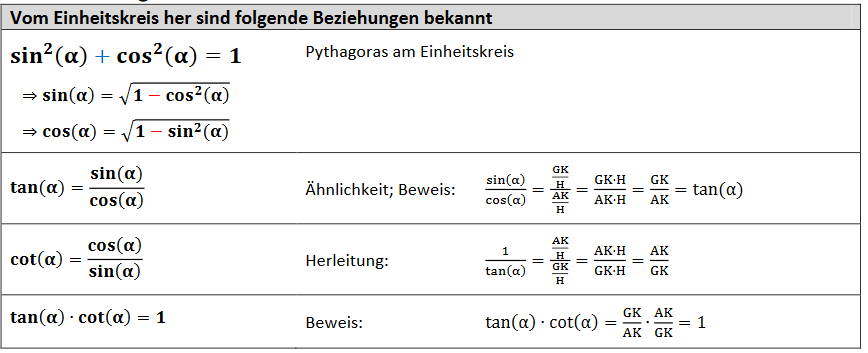
\includegraphics[scale=0.7]{gon1.PNG}

\subsubsection{Additionstheoreme}
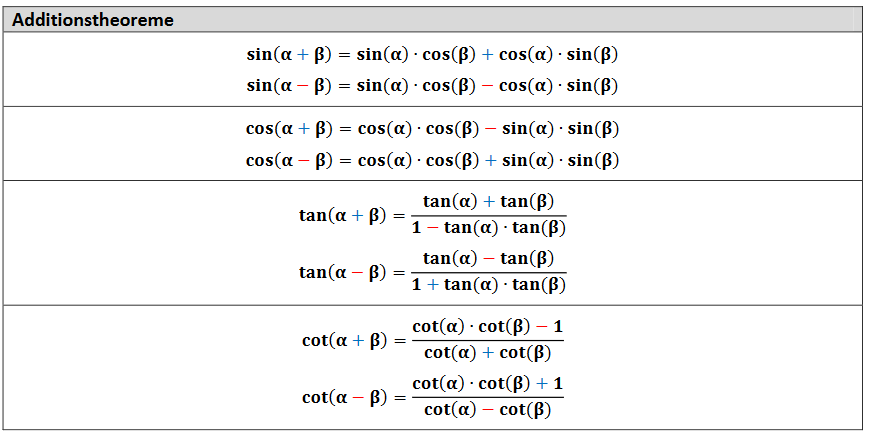
\includegraphics[scale=0.7]{gon2.PNG}

\subsubsection{Winkelfunktionen des doppelten Winkels}
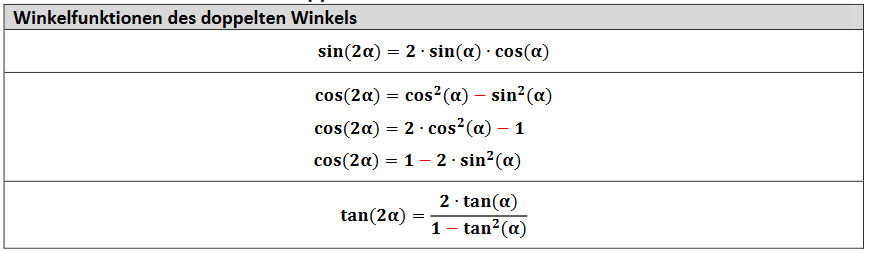
\includegraphics[scale=0.7]{gon3.PNG}

\subsubsection{Winkelfunktionen des dreifachen Winkels}
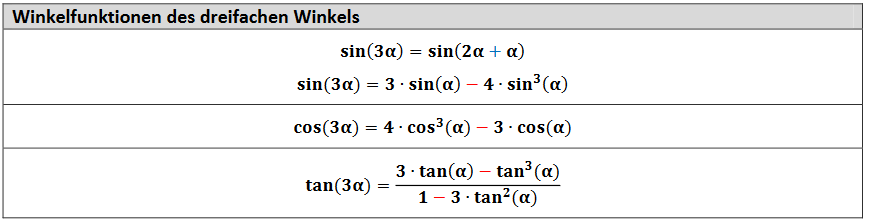
\includegraphics[scale=0.7]{gon4.PNG}

\subsubsection{Winkelfunktionen des halben Winkels}
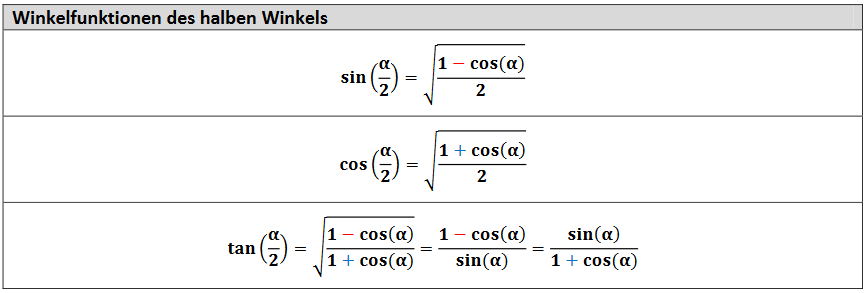
\includegraphics[scale=0.7]{gon5.PNG}

\section{Vektorgeometrie}
\subsection{Grunddefinitionen}
\textbf{Vektor:}

Ein Vektor ist festgelegt durch eine Laenge (Groesse) und eine Richtung.

\textbf{Freie Vektoren: }
Sie beschreiben Merkmale,
bei denen es nur auf Groesse und Richtung ankommt

\textbf{Ortsvektoren:}
Sie beschreiben Merkmale,
bei denen es auf Groesse, Richtung und Anfangspunkt ankommt

Unter einem Ortsvektor $\vec{v}$  versteht man eine Strecke, bei der der eine der beiden Begrenzungspunkte als Anfangspunkt P, der andere Endpunkt Q festgelegt ist. Man schreibt $\vec{v} = \vec{PQ}$

\subsection{Grundrechenarten}
\subsubsection{Addition von Vektoren}
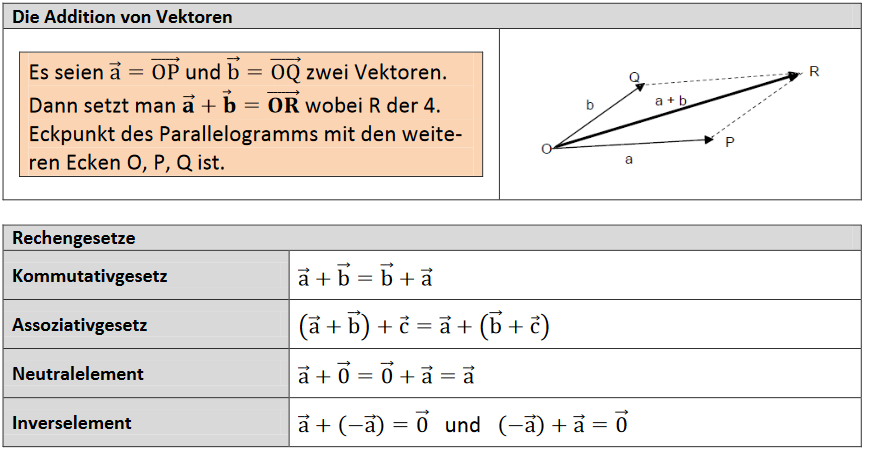
\includegraphics[scale=0.7]{vec1.PNG}
\subsubsection{Subtraktion von Vektoren}
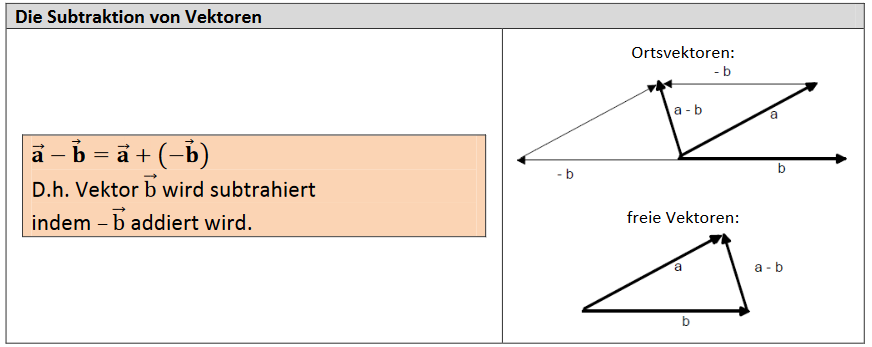
\includegraphics[scale=0.7]{vec2.PNG}
\subsubsection{Multiplikation mit einer Zahl}
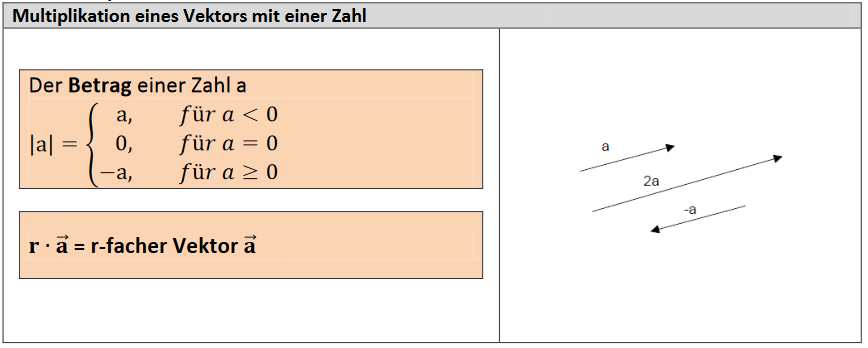
\includegraphics[scale=0.7]{vec3.PNG}

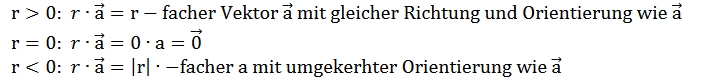
\includegraphics[scale=0.7]{vec3-1.PNG}

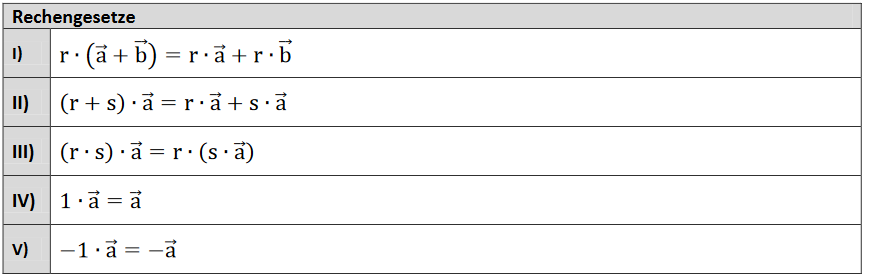
\includegraphics[scale=0.7]{vec3-2.PNG}

\subsubsection{Skalarprodukt}
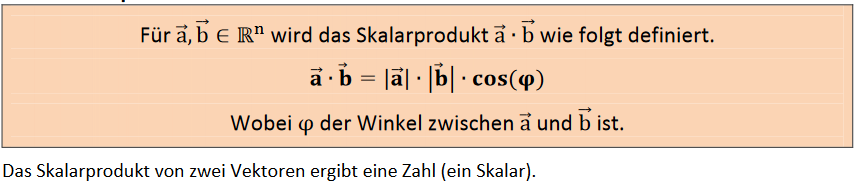
\includegraphics[scale=0.7]{vec4.PNG}

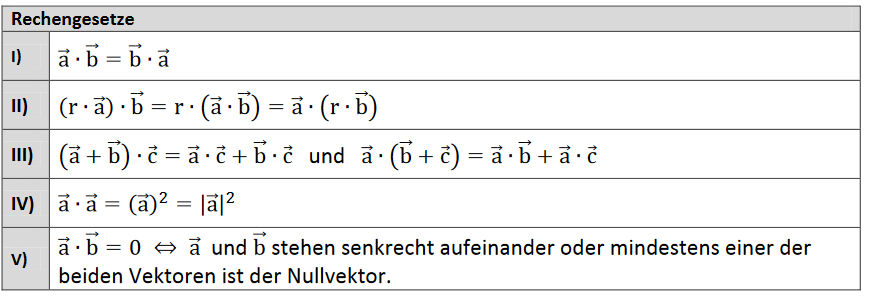
\includegraphics[scale=0.7]{vec4-1.PNG}

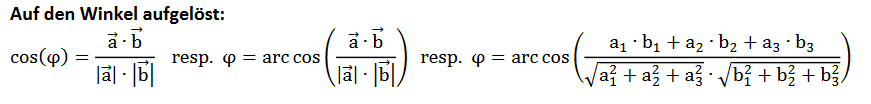
\includegraphics[scale=0.7]{vec4-2.PNG}

\subsubsection{Vektorprodukt}
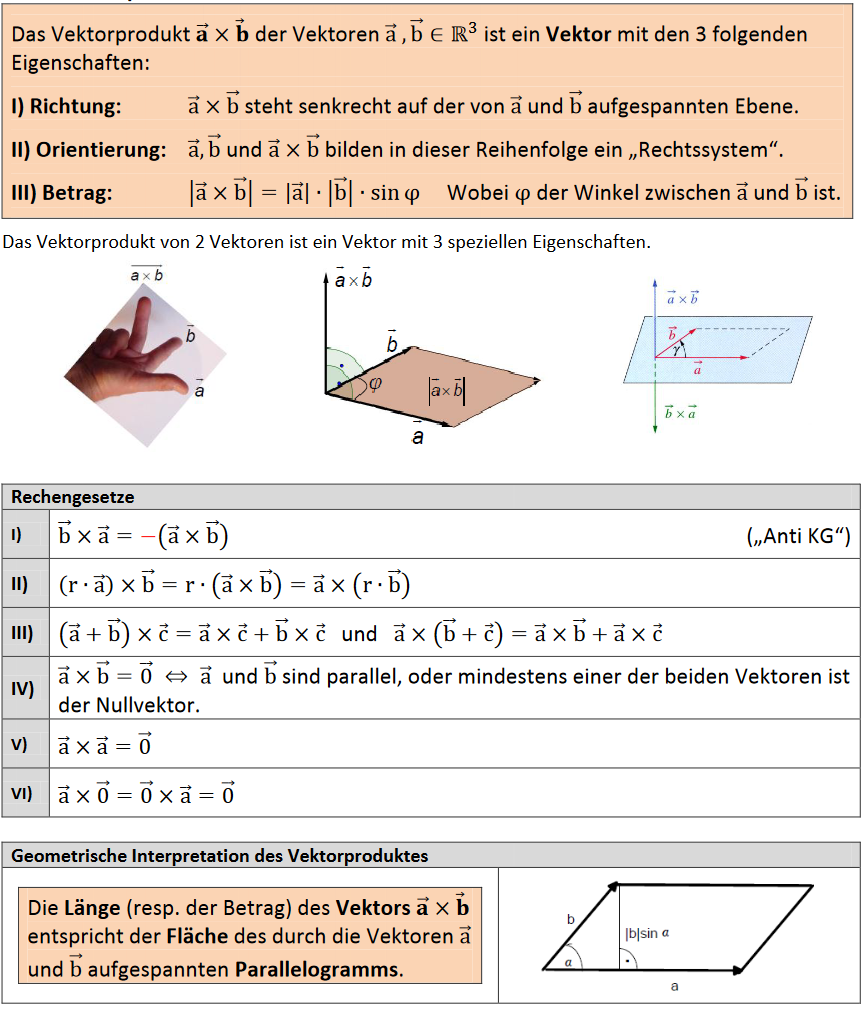
\includegraphics[scale=0.7]{vec5.PNG}
\newpage{}
\begin{multicols*}{2}
    \subsubsection{Betrag eines Vektors}
    Die Laenge eines Vektors heisst Betrag des Vektors.
    \[\vec{v}= \begin{pmatrix} x \\ y \end{pmatrix} \Longrightarrow \left|\vec{v}\right| = \sqrt{x^2 + y^2}\]
    \subsubsection{Einheitsvektor}
    Ein Vektor der Laenge heisst Einheitsvektor. \\
    Die Formel für die Berechnung des Einheitsvektors $\vec{a}^0$ lautet:
    \[\vec{a}^0 = \frac{1}{|a|} \vec{a}\]

    \subsection{Normalform}
    \subsubsection{Normalform einer Gerade}
    Eine Gerade laesst sich lediglich im $\mathbb{R}^2$ in Normalenform darstellen, weil es im $\mathbb{R}^3$ keinen eindeutigen Normalenvektor gibt.
    \[g\colon\; \vec{n} \circ [\vec{x} - \vec{a}] = 0\]

    \begin{itemize}
        \item  $\vec{g}$: Bezeichnung der Gerade
        \item  $\vec{n}$: Normalenvektor (Vektor, der senkrecht auf der Gerade steht)
        \item  $\vec{a}$: Aufpunkt (oder: Stuetzvektor)
    \end{itemize}
    \subsubsection{Normalform einer Ebene}
    \[E\colon\; \vec{n} \circ [\vec{x} - \vec{a}] = 0\]

    \begin{itemize}
        \item  $\vec{E}$: Bezeichnung der Ebene
        \item  $\vec{n}$: Normalenvektor (Vektor, der senkrecht auf der Gerade steht)
        \item  $\vec{a}$: Aufpunkt (oder: Stuetzvektor)
    \end{itemize}
    \subsubsection{Hessesche Normalform einer Gerade}
    \[g\colon\; \vec{n}_0 \circ [\vec{x} - \vec{a}] = 0\]
    \begin{itemize}
        \item  $\vec{n}$: Normalenvektor (Vektor, der auf einer Gerade senkrecht steht)
        \item  $\vec{n}_0$: Normierter Normalenvektor (Normalenvektor der Länge 1) $\vec{n}_0 = \frac{\vec{n}}{|\vec{n}|}$
        \item  $|\vec{n}|$: Laenge des Normalenvektors
        \item  $\vec{a}$: Aufpunkt (oder: Stuetzvektor)
    \end{itemize}

    Gegeben sei die Gerade g in Normalenform mit

    \[g\colon\; \vec{n} \circ \left[\vec{x} - \vec{a}\right] = \begin{pmatrix} 4 \\ 3 \end{pmatrix} \circ \left[\begin{pmatrix} x_1 \\ x_2 \end{pmatrix} - \begin{pmatrix} 2 \\ 1 \end{pmatrix}\right] = 0\]
    Länge des Normalenvektors berechnen:
    \[ |\vec{n}| = \sqrt{4^2 + 3^2} = \sqrt{25} = 5\]
    Gerade in Hessescher Normalform aufstellen
    \[g\colon\; \frac{\vec{n}}{|\vec{n}|} \circ \left[\vec{x} - \vec{a}\right] = \frac{1}{5} \cdot \begin{pmatrix} 4 \\ 3 \end{pmatrix} \circ \left[\begin{pmatrix} x_1 \\ x_2 \end{pmatrix} - \begin{pmatrix} 2 \\ 1 \end{pmatrix}\right] = 0\]

    Oder Gegeben sei die Gerade n in Koordinatenform mit:
    \[g\colon\; 4x_1 - 3x_2 - 5 = 0\]
    Normalenvektor aus Koordinatenform herauslesen

    Die Koordinaten des Normalenvektors entsprechen den Koeffizienten von $x_1$ und $x_2$ in der Koordinatenform.
    \[\vec{n} = \begin{pmatrix} 4 \\ -3 \end{pmatrix}\]
    Laenge des Normalenvektors berechnen
    \[|\vec{n}| = \sqrt{4^2 + (-3)^2} = \sqrt{25} = 5\]
    Gerade in Hessescher Normalform aufstellen
    \[g\colon\; \frac{1}{5} \cdot [4x_1 - 3x_2 - 5] = 0\]

    \subsubsection{Hessesche Normalform einer Ebene}
    \[E\colon\; \vec{n}_0 \circ [\vec{x} - \vec{a}] = 0\]
    \begin{itemize}
        \item  $\vec{n}$: Normalenvektor (Vektor, der auf einer Ebene senkrecht steht)
        \item  $\vec{n}_0$: Normierter Normalenvektor (Normalenvektor der Länge 1) $\vec{n}_0 = \frac{\vec{n}}{|\vec{n}|}$
        \item  $|\vec{n}|$: Laenge des Normalenvektors
        \item  $\vec{a}$: Aufpunkt (oder: Stuetzvektor)
    \end{itemize}
    Gegeben sei die Ebene E in Normalenform mit
    \[E\colon\; \vec{n} \circ \left[\vec{x} - \vec{a}\right] = \begin{pmatrix} 2 \\ 1 \\ -2 \end{pmatrix} \circ \left[\begin{pmatrix} x_1 \\ x_2 \\ x_3 \end{pmatrix} - \begin{pmatrix} 0 \\ 1 \\ 1 \end{pmatrix}\right] = 0\]
    Laenge des Normalenvektors berechnen
    \[|\vec{n}| = \sqrt{2^2 + 1^2 + (-2)^2} = \sqrt{9} = 3\]
    Ebene in Hessescher Normalform aufstellen
    \[E\colon\; \frac{\vec{n}}{|\vec{n}|} \circ \left[\vec{x} - \vec{a}\right] = \frac{1}{3} \cdot \begin{pmatrix} 2 \\ 1 \\ -2 \end{pmatrix} \circ \left[\begin{pmatrix} x_1 \\ x_2 \\ x_3 \end{pmatrix} - \begin{pmatrix} 0 \\ 1 \\ 1 \end{pmatrix}\right] = 0\]

\end{multicols*}

\newpage{}
